\documentclass{article}
\usepackage{amsmath}
\usepackage{amssymb}
\usepackage{graphicx}
\usepackage{hyperref}
\usepackage[version=4]{mhchem}

\title{Example 3}
\date{}

\begin{document}
\maketitle

In \(\triangle A B C\), point \(E\) is the midpoint of \(A C\). \(D\) is on \(B C\) and \(B D=1 / 3\) \(B C\). Show that \(A D\) bisects \(B E\).

Solution:
Method 1:\\
Let the point of intersection of \(B E\) and \(A D\) be \(P\).\\
\centering
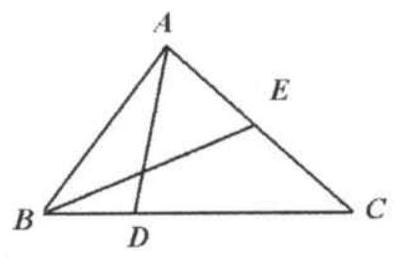
\includegraphics[width=\textwidth]{images/036(1).jpg}

Connect \(E F\) where \(F\) is the midpoint of \(D C\).\\
Since \(E\) is the midpoint of \(A C\) and \(F\) is the midpoint of \(D C, A D / / E F\).\\
Therefore \(E F=\frac{1}{2} A D\).\\
\centering
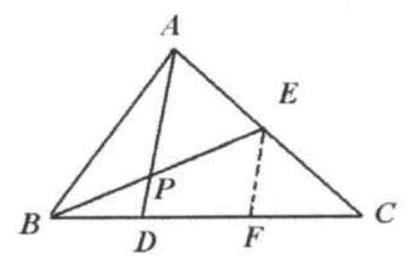
\includegraphics[width=\textwidth]{images/036.jpg}

In \(\triangle B E F, P D / / E F, B D=D F\). Therefore \(P D\) bisects BE , or in other words, \(A D\) bisects \(B E\).

Method 2:\\
Draw \(E G / / D C\) to meet \(A D\) at \(G\).\\
\centering
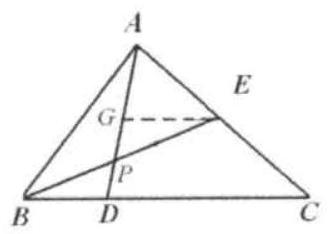
\includegraphics[width=\textwidth]{images/036(3).jpg}


Since point \(E\) is the midpoint of \(A C\), by Theorem 2.2, \(G\) is the midpoint of \(A D\) and \(E G=\frac{1}{2} D C\).\\
We know that \(B D=1 / 3 B C\). So \(D C=\frac{2}{3} B C\) and \(E G=\frac{1}{2} D C=\frac{1}{2} \times \frac{2}{3} B C=\) \(\frac{1}{3} B C=B D\).\\
Thus \(\triangle E G P \cong \triangle B D P(E G=B D, \angle G E P=\angle D B P\) and \(\angle G E P=\angle D B P)\). So \(B P=P E\). In other words, \(A D\) bisects \(B E\).


\end{document}
